\section{Introduction}\label{sec:intro}
% Variant B intro (one central limitation + research-question hinge), per playbook §1.
% Ledger: see ledger.md. Numbers quoted here are single-run; refresh after E2 medians.
A graph represents entities as vertices and their pairwise relationships as edges.
%
Groups of vertices that are densely connected to one another often carry the meaning of the whole network.
%
For example, in collaboration networks, dense groups correspond to research teams working closely together \cite{girvan2002community}; in web graphs, they mark clusters of pages on one topic \cite{gibson1998inferring}; in biological networks, they capture protein complexes \cite{sharan2006modeling}; in financial and social platforms, they expose coordinated fraud rings \cite{akoglu2015graph,jiang2016catching}.

Decomposing a graph into a hierarchy of nested dense subgraphs is a fundamental task in graph mining.
%
Representative applications include community detection \cite{girvan2002community,rossetti2019community}, densest-subgraph discovery \cite{tsourakakis2013finding}, influence analysis \cite{kempe2003maximizing,li2015influential}, and graph visualization \cite{malliaros2013clustering}.
%
In the literature, the task has been studied at three levels of granularity.
%
The $k$-core peels vertices by degree \cite{seidman1983network,batagelj2011fast}; the $k$-truss peels edges by triangle count \cite{cohen2008trusses,wang2012truss}; the $(r,s)$-nucleus decomposition peels $r$-cliques by $s$-clique count \cite{firstNucleus}.
%
The nucleus model subsumes the other two: the $(1,2)$-nucleus is exactly the $k$-core, and the $(2,3)$-nucleus is exactly the $k$-truss \cite{firstNucleus}.
%
The parameter pair $(r,s)$ therefore acts as a resolution, and every cell of the parameter plane reveals the graph's dense structure at a different granularity \cite{firstNucleus,nuclearTWEB}.
%
The state-of-the-art algorithm, \cnd~\cite{NuclearCD}, computes the decomposition of one cell at a time.
%
In this paper, we aim to answer every cell of a bounded parameter plane from one index.

For integers $r<s$, consider subgraphs in which every $r$-clique is contained in at least $k$ $s$-cliques of the same subgraph.
%
The nucleus value of an $r$-clique is the largest $k$ for which such a subgraph contains it.
%
Computing the cell $(r,s)$ means computing this value for every $r$-clique of the graph.

\begin{figure}[t]
    \centering
    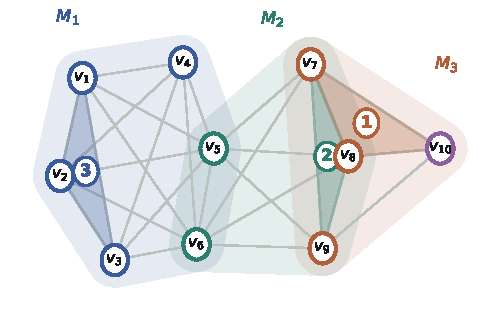
\includegraphics[width=0.96\linewidth]{figures/fig1_example.pdf}
    \caption{An example graph $G$ and three of its $(3,4)$-nucleus values.}
    \label{fig:example}
\end{figure}

\begin{example}\label{exa:running}
Consider the graph $G$ in Figure~\ref{fig:example}, whose ten vertices form three maximal cliques: $M_1$ with six vertices, $M_2$ with five, and $M_3$ with four.
%
At the cell $(3,4)$, the triangle $\{v_1,v_2,v_3\}$ has nucleus value $3$: it lies in the subgraph induced by $M_1$, in which every triangle is contained in at least three $4$-cliques.
%
The triangle $\{v_7,v_8,v_9\}$ has value $2$, and the triangle $\{v_7,v_8,v_{10}\}$ has value $1$.
%
Other cells give other resolutions: at $(3,5)$ the value of $\{v_1,v_2,v_3\}$ is still $3$, while at $(4,5)$ the $4$-clique $\{v_1,v_2,v_3,v_4\}$ has value $2$.
\end{example}

\stitle{Applications.}
Many uses of the decomposition need several cells of the plane rather than one.
%
\sstitle{Multi-resolution exploration.}
An analyst inspecting a dense region rarely knows the right resolution in advance.
%
Low cells surface broad communities, while high cells isolate small, strongly coordinated groups \cite{firstNucleus,jiang2016catching}.
%
Exploration therefore issues a stream of queries across cells, and each query must return in interactive time.
%
\sstitle{Parameter selection.}
Which cell best separates signal from noise differs across graphs and tasks \cite{nuclearTWEB}.
%
Practitioners choose by probing: compute several cells, compare the resulting hierarchies, and keep the most informative one.
%
Today every probe costs a full decomposition run.
%
\sstitle{Point queries at query time.}
Downstream systems ask point questions: given one concrete group of vertices, how dense is its surrounding structure at each resolution \cite{huang2014graph}?
%
Answering from the raw graph requires a fresh decomposition per question.

\stitle{Existing Methods and Key Limitation.}
The state-of-the-art algorithm \cnd~\cite{NuclearCD} enumerates every $r$-clique of the requested cell, counts its supporting $s$-cliques, and repeatedly removes the clique of minimum count.
%
Careful counting structures let it obtain these counts without listing individual $s$-cliques, which made single-cell decomposition practical on graphs with millions of edges \cite{NuclearCD}.
%
However, all existing algorithms share a fundamental limitation: they materialize \textbf{\textit{every $r$-clique of every cell they compute}}.
%
The number of $r$-cliques grows combinatorially with $r$: \webit, a web graph with $7.2$ million edges, contains more than $1.5\times10^{12}$ $5$-cliques.
%
Even a single shallow cell is already prohibitive: on \webit, \cnd{} needs $5{,}581$ seconds and $101$\,GB of memory for the single cell $(3,4)$.
%
Within a $1{,}800$-second, $300$\,GB budget, \cnd{} finishes none of the nine \webit{} cells of our evaluation grid (Section~\ref{sec:experiments}).

This leads to the central research question of this paper: \textbf{\textit{Can one index answer the nucleus value of every $r$-clique, at every cell of a bounded plane, without ever materializing the plane?}}

\stitle{Challenges.}
Answering the plane from one structure faces three obstacles.
%
\sstitle{Astronomically many objects.}
For one small cell, per-clique computation is affordable.
%
However, across a plane the objects multiply twice: the number of $r$-cliques explodes with $r$, and every cell owns its own copy of the work.
%
Even the ten-vertex graph of Figure~\ref{fig:example} carries $61$ cliques of size three to five; on \webit{} the count exceeds $10^{12}$.
%
Therefore, any approach that touches each $r$-clique of each cell even once is ruled out from the start.
%
\sstitle{Counting without enumeration.}
Peeling is driven by counts: each removal must decrement the count of every $r$-clique that shared a supporting $s$-clique with the removed one.
%
However, $s$-cliques outnumber $r$-cliques, and at high $s$ they cannot even be listed once.
%
Therefore, both the initial counts and every later decrement must be obtained without enumerating a single $s$-clique.
%
\sstitle{A plane of cells.}
A bounded plane contains dozens of cells, and each cell is a full decomposition in its own right.
%
However, running even the best single-cell algorithm once per cell multiplies its cost by the number of cells.
%
Worse, the deep cells are exactly the ones no existing algorithm reaches.
%
Therefore, the computation done in one cell must be made to pay for all the others.

\stitle{Our Idea.}
Our solution is built on one structural observation: vertices that belong to exactly the same maximal cliques are interchangeable, and the whole plane respects this symmetry.
%
We call the resulting grouping the \textit{clique quotient} of the graph.
%
\sstitle{Peel patterns, not cliques.}
Under the quotient, an $r$-clique is described by how many vertices it takes from each group, not by which vertices it takes.
%
The $33$ triangles of Figure~\ref{fig:example} collapse into $7$ such patterns; on real graphs the collapse reaches six orders of magnitude.
%
The peel runs unchanged on patterns, with every step carrying a multiplicity.
%
\sstitle{Count as a coefficient.}
The number of $s$-cliques containing a pattern is a coefficient of one small polynomial derived from the quotient.
%
Both the initial counts and all later decrements reduce to coefficient extraction, so no $s$-clique is ever listed.
%
\sstitle{Certify instead of recompute.}
Two transfer theorems link neighboring cells.
%
Along $s$, a pattern whose value reaches its closed form keeps that form in every later cell.
%
Along $r$, the starting values of a cell follow from the cell below it.
%
Together they leave a single cell to peel; every other cell of the plane is arithmetic.

The consequence is an index that stores almost nothing.
%
Wherever the closed form is certified, the value is reconstructed at query time from the quotient itself, so certified patterns cost zero bytes.
%
We call the structure \nsi, for \underline{N}ucleus \underline{S}pectrum \underline{I}ndex.

\stitle{Contributions.}
Our key contributions are summarized as follows.
%
\sstitle{The first index over the nucleus plane.}
We propose \nsi{} (Section~\ref{sec:index}), the first index that answers every cell of a bounded $(r,s)$ plane from one structure.
% TODO(thm-ref): upgrade the section reference to the reconstruction lemma once labeled.
On \webit, the explicit table behind the same queries would occupy $46.2$\,TB, and it cannot be built at all for $r\ge4$.
%
\nsi{} occupies $1.66$\,MB and answers a point query in $74$ nanoseconds.
%
\sstitle{A quotient framework with certified transfer.}
We develop the clique quotient and its peel (Sections~\ref{sec:quotient}--\ref{sec:plane}): interchangeability, coefficient counting, and two transfer certificates that reduce the whole plane to one peeled cell.
% TODO(thm-ref): cite the interchangeability theorem, coefficient lemma, and the two certificates.
Disabling the certificates alone slows the build by $22.6\times$ on \nasasrb, with answers unchanged.
%
\sstitle{An applicability test computable in advance.}
We characterize exactly when the quotient compresses, by a one-number test computable before any index is built (Section~\ref{sec:index}).
%
The test predicted every graph of our evaluation, and it also predicted the social networks the evaluation excludes.
%
On \pokec{} the quotient compresses by a factor of only $1.001$, and the test reports this without building anything.
%
\sstitle{Comprehensive Experimental Evaluation.}
We evaluate on eight graphs from four domains, all with at least a million edges (Section~\ref{sec:experiments}).
%
Against \cnd{} run serially on the same machine, our builder wins every cell of the evaluation grid, by up to $742\times$ in time and $226\times$ in memory.
%
It also completes the deep cells on which \cnd{} exceeds every budget.
% TODO(avg): add the average speedup once multi-trial medians (E2) land.
